% CompToolBench Paper — NeurIPS 2026 Datasets & Benchmarks Track
% Use [preprint] for ArXiv, remove for blind submission
\documentclass{article}
\usepackage[preprint,dandb]{neurips_2025}

% ── Packages ──────────────────────────────────────────────────────────
\usepackage[utf8]{inputenc}
\usepackage[T1]{fontenc}
\usepackage{hyperref}
\usepackage{url}
\usepackage{booktabs}
\usepackage{amsfonts}
\usepackage{amsmath}
\usepackage{nicefrac}
\usepackage{microtype}
\usepackage{graphicx}
\usepackage{subcaption}
\usepackage{xcolor}
\usepackage{enumitem}
\usepackage{multirow}
\usepackage{colortbl}
\usepackage{float}
\usepackage{tikz}
\usetikzlibrary{positioning, arrows.meta}

% ── Colors (Okabe-Ito palette for accessibility) ─────────────────────
\definecolor{cL0}{HTML}{0072B2}
\definecolor{cL1}{HTML}{009E73}
\definecolor{cL2}{HTML}{E69F00}
\definecolor{cL3}{HTML}{D55E00}
\definecolor{cgap}{HTML}{CC79A7}
\definecolor{ccloud}{HTML}{56B4E9}
\definecolor{clocal}{HTML}{999999}

% ── Custom commands ──────────────────────────────────────────────────
\newcommand{\bench}{\textsc{CompToolBench}}
\newcommand{\compgap}{\textsc{CompGap}}
\newcommand{\selgap}{\textsc{SelGap}}
\newcommand{\lzero}{$\text{L}_0$}
\newcommand{\lone}{$\text{L}_1$}
\newcommand{\ltwo}{$\text{L}_2$}
\newcommand{\lthree}{$\text{L}_3$}
\newcommand{\pp}{\text{pp}}

% ═════════════════════════════════════════════════════════════════════
\title{\bench{}: Measuring the Compositional Tool-Use Gap\\in Large Language Models}

\author{
  Md A Rahman \\
  Texas Tech University \\
  \texttt{ara02434@ttu.edu} \\
}

\begin{document}
\maketitle

% ─────────────────────────────────────────────────────────────────────
\begin{abstract}
Large language models now routinely call external tools, yet existing benchmarks evaluate \emph{isolated} tool calls, implicitly assuming that single-tool proficiency is the ``easy'' baseline from which performance degrades as tasks grow more complex.
We introduce \bench{}, a controlled benchmark comprising 200 tasks across 106 deterministic tool simulations at four composition levels: single calls (\lzero{}), sequential chains (\lone{}), parallel fork-join patterns (\ltwo{}), and directed acyclic graphs (\lthree{}).
Evaluating 18 models (10 cloud API, 8 local) across 6 inference providers, we identify the \emph{Selection Gap}: 17 of 18 models score \emph{higher} on composed multi-tool tasks than on isolated single-tool selection, with an average gap of 13.2 percentage points~(pp) (19.9\,$\pp$ among cloud models, 4.7\,$\pp$ among local models).
The most extreme case, Llama~3.1~8B on Groq, achieves only 27.1\% on \lzero{} but 79.6\% on average across \lone{}--\lthree{}.
We observe three additional patterns:
\textbf{(1)}~Parallel composition (\ltwo{}) is easier than sequential across the full evaluation (67.3\% vs.\ 58.0\%), but this holds only among cloud models (80.5\% vs.\ 59.7\%); local models show the opposite pattern (\ltwo{} $<$ \lone{}), a divergence we trace to inference infrastructure differences.
\textbf{(2)}~The traditional L$_0$-to-L$_3$ composition gap remains modest (5.8\,$\pp$ overall, and only 0.6\,$\pp$ among cloud models) once tool selection is tested with natural-language prompts against a realistic 106-tool catalog, compared to 26.8\,$\pp$ in our V1 evaluation with 43 tools.
\textbf{(3)}~A weight-ablation study over 8 scoring configurations shows that model rankings are stable (Spearman $\rho \geq 0.83$ for 6 of 7 alternative weightings) and the Selection Gap persists under all non-degenerate scoring configurations.
All code, data, and evaluation infrastructure are publicly available.\footnote{\url{https://github.com/ronyrahmaan/comptoolbench}}
\end{abstract}

% ─────────────────────────────────────────────────────────────────────
\section{Introduction}
\label{sec:intro}

Equipping language models with external tool calls has become a standard design pattern for AI agents~\citep{schick2024toolformer,patil2023gorilla}.
From web browsing to code execution, function calling allows LLMs to take actions beyond text generation.
Real-world tasks, however, rarely require a single tool call in isolation; they demand \emph{compositional} reasoning---chaining outputs, parallelizing sub-tasks, and routing data through branching pipelines.

Existing tool-use benchmarks~\citep{berkeley2024bfcl,li2023apibank,qin2024toolllm} primarily evaluate whether a model can identify \emph{which} tool to use and supply \emph{correct arguments} for a single function call.
These benchmarks implicitly assume that single-tool selection is the ``easy'' baseline and that performance degrades as task complexity increases.
\bench{} was designed to test this assumption directly, by systematically varying composition structure while holding tool difficulty constant.

\bench{} is built around four composition levels, each representable as a directed acyclic graph (DAG):

\begin{enumerate}[nosep,leftmargin=*]
    \item \textbf{\lzero{} (Single):} One tool call from a natural-language prompt---the baseline.
    \item \textbf{\lone{} (Chain):} Sequential calls where each step depends on the previous output.
    \item \textbf{\ltwo{} (Parallel):} Independent calls executed concurrently, followed by aggregation.
    \item \textbf{\lthree{} (DAG):} Branching and merging patterns combining sequential and parallel elements.
\end{enumerate}

A key design choice is that \lzero{} tasks use \emph{natural-language} prompts (``What is the weather like in Paris?'') against the full 106-tool catalog, rather than explicit tool-name instructions.
This mirrors how real users interact with tool-augmented assistants and exposes a failure mode invisible to benchmarks that specify tool names explicitly.

Our evaluation of 18 models (10 cloud API, 8 local) across 6 inference providers yields an \textbf{unexpected result}:

\begin{quote}
\textbf{The Selection Gap.}
17 of 18 models achieve \emph{higher} accuracy on composed multi-tool tasks (\lone{}--\lthree{}) than on isolated single-tool selection (\lzero{}).
On average, \lzero{} accuracy is 40.0\%, while the composed average (\lone{}--\lthree{}) is 53.2\%, a gap of 13.2\,$\pp$ in the \emph{wrong} direction (19.9\,$\pp$ among cloud models).
\end{quote}

This result calls into question the common assumption that isolated tool selection is the ``easy'' case.
When models face realistic tool catalogs with natural-language queries, selecting the right tool from 106 options is \emph{harder} than composing multiple tools in a multi-step workflow.
The richer task descriptions in composed prompts provide contextual cues that narrow the search space.

Three further results clarify this finding:

\begin{enumerate}[nosep,leftmargin=*]
    \item \textbf{Parallel composition is easier than sequential, but only for cloud models.}
    Across all 18 models, \ltwo{} (parallel, avg.\ 67.3\%) outperforms \lone{} (sequential, avg.\ 58.0\%).
    However, this holds only among cloud models (80.5\% vs.\ 59.7\%); local models show the \emph{opposite} pattern (50.8\% vs.\ 55.8\%), consistent with the hypothesis that optimized cloud inference particularly helps with parallel tool dispatch.

    \item \textbf{The traditional composition gap remains modest.}
    The average L$_0 \rightarrow $ L$_3$ delta is 5.8\,$\pp$ overall (and only 0.6\,$\pp$ among cloud models), compared to 26.8\,$\pp$ in our V1 evaluation with 43 tools.
    Earlier benchmarks' small tool inventories may have inflated L$_0$ accuracy, making tool selection appear easier than it is at realistic catalog sizes.

    \item \textbf{Results are stable across scoring methodologies.}
    An ablation across 8 weight configurations yields Spearman rank correlations of $\rho \geq 0.83$ for 6 of 7 alternative weightings, and the gap persists under all non-degenerate configurations tested.
\end{enumerate}

\noindent Our contributions are:
\begin{enumerate}[nosep,leftmargin=*]
    \item A \textbf{controlled benchmark} with 200 tasks across 106 tools at 4 DAG-based composition levels, with deterministic tool simulations for bit-exact reproducibility.
    \item A \textbf{fine-grained scoring system} decomposing performance into tool selection, argument accuracy, data flow, and completeness, validated through an 8-configuration ablation study.
    \item The \textbf{\selgap{} finding}: controlled evidence that single-tool selection from natural-language prompts can be systematically harder than composed multi-tool execution, and the \compgap{} metric that quantifies this relationship.
    \item A \textbf{systematic evaluation of 18 models} (10 cloud, 8 local) across 6 providers, documenting the near-universal Selection Gap and a systematic cloud--local split in parallel composition.
\end{enumerate}

% ─────────────────────────────────────────────────────────────────────
\section{Related Work}
\label{sec:related}

\paragraph{Single-tool benchmarks.}
The Berkeley Function Calling Leaderboard (BFCL~V4)~\citep{berkeley2024bfcl} evaluates function calling via AST matching and recently added multi-turn agentic evaluation, but does not systematically vary composition structure or measure the accuracy delta between single and composed calls.
APIBench~\citep{patil2023gorilla} and ToolBench~\citep{qin2024toolllm} focus on API selection from large catalogs (16,000+ APIs) without compositional variation; StableToolBench~\citep{qin2024stabletoolbench} improves evaluation stability but inherits this single-tool focus.

\paragraph{Multi-tool and compositional benchmarks.}
Several recent works test compositional tool use.
\textbf{FuncBenchGen}~\citep{maekawa2025funcbenchgen}, accepted at ICLR 2026, shares our DAG formulation and controls difficulty via graph depth, but uses \emph{synthetic} functions rather than real APIs and lacks an explicit composition gap metric.
\textbf{ComplexFuncBench}~\citep{zhao2025complexfuncbench} tests multi-step function calling across 43 real-time APIs in long-context scenarios (128K tokens) but does not distinguish chain vs.\ parallel vs.\ DAG patterns.
\textbf{TPS-Bench}~\citep{wu2025tpsbench} evaluates tool planning and scheduling in compounding tasks, focusing on time-optimization rather than accuracy across topology levels.
ToolComp~\citep{scale2024toolcomp} tests dependent tool use with process supervision but uses only 11 tools.
NESTful~\citep{li2024nestful} tests nested sequences but restricts composition to sequential nesting.
Nexus~\citep{nexusflow2024nexusbench} defines three categories (single, parallel, nested) with 762 test cases---a simpler taxonomy than our four-level hierarchy.

\paragraph{MCP-ecosystem benchmarks.}
A growing family of benchmarks targets the Model Context Protocol ecosystem:
MCP-Bench~\citep{accenture2025mcpbench} tests 250 tools across 28 servers,
MCPAgentBench~\citep{zhang2025mcpagentbench} scales to 20K+ tools with distractor selection,
and LiveMCPBench~\citep{wang2025livemcpbench} evaluates 527 tools in dynamic environments.
These focus on a specific protocol ecosystem; \bench{} is protocol-agnostic and measures compositional accuracy across explicit topology levels.

\paragraph{Interactive and real-world benchmarks.}
WildToolBench~\citep{huang2025wildtoolbench} reports that no model exceeds 15\% on realistic multi-tool scenarios---a finding consistent with the low \lzero{} accuracy we observe.
ToolSandbox~\citep{apple2024toolsandbox} evaluates stateful conversational tool use,
and OpaqueToolsBench~\citep{chen2025opaquetoolsbench} tests learning to use underspecified tools---challenges orthogonal to compositional structure.
TOP-Bench~\citep{liu2025topbench} examines privacy risks from tool orchestration, finding 90\% leakage rates, a complementary safety dimension.

\paragraph{How \bench{} differs.}
\bench{} differs in three ways.
First, it controls composition structure across four DAG-based levels (L$_0$--L$_3$) with 106 deterministic tool simulations spanning 15 categories.
Second, it introduces the \compgap{} metric and evaluates 18 models across 6 providers (cloud API and local Ollama) at zero marginal cost.
Third, it provides controlled evidence that natural-language tool selection can be harder than composed multi-tool execution.

\paragraph{Compositional generalization.}
The broader challenge of compositional generalization has been studied extensively~\citep{lake2018generalization,keysers2020measuring}.
COGS~\citep{kim2020cogs} and SCAN~\citep{lake2018generalization} demonstrate that neural models often fail to recombine known primitives in novel ways.
We adapt this framing to tool use and find that, given a realistic tool catalog, the primary difficulty is tool disambiguation, not composition.

\paragraph{LLM agents.}
Agentic frameworks like ReAct~\citep{yao2023react}, Toolformer~\citep{schick2024toolformer}, and various architectures~\citep{wang2024survey} rely on compositional tool use as a core capability.
\bench{} provides a controlled testbed for this capability in isolation, without confounds from environment interaction or multi-turn dialogue.

% ─────────────────────────────────────────────────────────────────────
\section{The \bench{} Benchmark}
\label{sec:benchmark}

\subsection{Design Principles}
\label{sec:design}

\bench{} is built on three principles:

\textbf{1.~Controlled composition.}
Every task is defined by a DAG specifying the exact sequence, parallelism, and data flow between tool calls.
Controlled composition allows us to isolate composition structure as the independent variable while holding tool selection difficulty constant.

\textbf{2.~Deterministic evaluation.}
All 106 tools support a \emph{simulated mode} that produces deterministic outputs from a hash of the input arguments.
Results therefore reproduce exactly without live API access, avoiding confounds from API instability or rate limits.

\textbf{3.~Realistic tool selection.}
\lzero{} tasks use natural-language prompts (e.g., ``What is the weather in Tokyo?'') against the full 106-tool catalog, forcing models to disambiguate among semantically similar tools, as real users do not specify tool names.

\subsection{Tool Inventory}
\label{sec:tools}

\bench{} includes 106 tools organized into 15 functional categories (Table~\ref{tab:tool_categories} in Appendix):
\emph{Math \& Statistics} (12 tools),
\emph{Text Processing} (10),
\emph{External Services} (9),
\emph{Data Operations} (8),
\emph{Web \& Network} (8),
\emph{String Utilities} (7),
\emph{Date \& Time} (7),
\emph{Communication} (7),
\emph{Encoding \& Security} (6),
\emph{Information Retrieval} (6),
\emph{File \& Data} (6),
\emph{Formatting} (5),
\emph{Productivity} (5),
\emph{AI \& NLP} (5),
and \emph{State Management} (5).
Each tool has a full OpenAI function-calling schema with typed parameters and realistic argument patterns.
The 200-task suite uses 58 unique tools; the remaining 48 serve as \emph{distractors} in the tool catalog, increasing the selection difficulty at \lzero{}.

\subsection{Composition Levels}
\label{sec:levels}

Tasks are generated deterministically by the \texttt{CompositionEngine} (seed 42) at four levels:

\textbf{\lzero{}: Single Call (48 tasks).}
The model must identify and invoke a single tool from the full 106-tool catalog given only a natural-language description.
Scoring is binary: a task passes if the correct tool is called with arguments achieving $\geq 0.85$ similarity.
The natural-language framing tests whether models can map vague human intent to the correct API endpoint, a harder task than selecting from a schema where the tool name is given in the prompt.

\textbf{\lone{}: Sequential Chain (64 tasks).}
Two tools called in sequence, where the second call's arguments depend on the first call's output.
Example: \texttt{lookup\_entity("Paris")} $\rightarrow$ \texttt{get\_weather(city="Paris")}.
The multi-step prompt implicitly narrows the tool search space, providing more context than an \lzero{} prompt.

\textbf{\ltwo{}: Parallel Fork-Join (40 tasks).}
Two or more independent tool calls followed by an aggregation step.
Example: \texttt{get\_weather("Tokyo")} $\|$ \texttt{get\_weather("London")} $\rightarrow$ \texttt{compare\_texts(...)}.
Parallel branches have \emph{no data dependency} on each other, so failures cannot cascade between branches.

\textbf{\lthree{}: DAG (48 tasks).}
Complex patterns combining sequential and parallel elements with branching and merging (4--6 tool calls).
Example: Fetch weather and stock data for two cities in parallel, convert currencies, then compose a summary email.

\subsection{Scoring System}
\label{sec:scoring}

Each task is scored along four dimensions:

\begin{enumerate}[nosep,leftmargin=*]
    \item \textbf{Tool Sequence Score}: Correctness of the tool call sequence, measured via longest common subsequence (LCS) ratio between predicted and expected sequences.
    \item \textbf{Argument Score}: Type-aware matching of arguments: exact match for strings, $\pm$1\% tolerance for numbers, fuzzy matching for natural language arguments.
    \item \textbf{Completeness Score}: Fraction of expected tool calls that were attempted.
    \item \textbf{Data Flow Score}: Whether outputs from earlier calls correctly feed into later calls' arguments.
\end{enumerate}

\lzero{} tasks use binary pass/fail scoring (correct tool $\wedge$ argument similarity $\geq 0.85$).
For \lone{}--\lthree{}, dimensions are combined with level-specific weights:
\lone{} weights sequence (0.40), arguments (0.35), completeness (0.25);
\ltwo{} adds data flow (0.35 seq, 0.35 args, 0.15 flow, 0.15 completeness);
\lthree{} emphasizes data flow further (0.30 seq, 0.30 args, 0.25 flow, 0.15 completeness).
The weighted combination yields a score in $[0, 1]$ per task.

The binary \lzero{} scoring is deliberately stricter than the weighted \lone{}--\lthree{} scoring, which \emph{amplifies} the Selection Gap: even with this disadvantage, \lzero{} would be expected to outperform composed levels if single-tool selection were truly ``easier.''
An ablation study (\S\ref{sec:ablation}) confirms that the Selection Gap persists across all scoring configurations.

\subsection{The Composition Gap Metric}
\label{sec:metric}

The \compgap{} for level $k$ measures the accuracy difference between single-tool and composed performance:
\begin{equation}
    \text{CompGap}_k = \text{Acc}_{L_0} - \text{Acc}_{L_k}
    \label{eq:compgap}
\end{equation}
A positive value indicates the expected compositional degradation; a \emph{negative} value indicates the Selection Gap---the model performs \emph{better} on composed tasks than isolated selection.
The overall \compgap{} is:
\begin{equation}
    \text{CompGap} = \frac{1}{3}\left(\text{CompGap}_{L_1} + \text{CompGap}_{L_2} + \text{CompGap}_{L_3}\right)
\end{equation}

% ─────────────────────────────────────────────────────────────────────
\section{Experimental Setup}
\label{sec:experiments}

\subsection{Models}
\label{sec:models}

We evaluate 18 models with native function-calling support across 6 inference providers (Table~\ref{tab:leaderboard}).
The evaluation spans two deployment regimes:

\textbf{Cloud API models (10).}
\begin{itemize}[nosep,leftmargin=*]
    \item \textbf{Groq:} Llama~3.1~8B, Llama~4~Scout~17B
    \item \textbf{Mistral API:} Mistral Small (${\sim}$22B), Mistral Medium, Mistral Large
    \item \textbf{OpenRouter:} Gemini~2.0~Flash
    \item \textbf{Cerebras:} Llama~3.1~8B, GPT-OSS~120B
    \item \textbf{Cohere:} Command~A, Command~R+
\end{itemize}

\textbf{Local models via Ollama (8).}
\begin{itemize}[nosep,leftmargin=*]
    \item Llama~3.1~8B, Mistral~7B, Mistral~Nemo~12B, Mistral~Small~24B
    \item Qwen3~8B, Qwen~2.5~7B, Granite4~3B, Granite4~1B
\end{itemize}

This design enables two controlled comparisons.
First, \emph{serving infrastructure}: Llama~3.1~8B is evaluated on Groq, Cerebras, and Ollama (identical weights, three providers), allowing us to compare the same model under three serving configurations.
Second, \emph{cloud vs.\ local deployment}: comparing optimized cloud APIs against local inference uncovers systematic differences in how models handle parallel composition.

\subsection{Evaluation Protocol}

\begin{enumerate}[nosep,leftmargin=*]
    \item \textbf{Task generation:} 200 tasks generated deterministically with seed 42 using the \texttt{CompositionEngine}, which constructs DAG-structured tasks from composable tool pairs.
    \item \textbf{Inference:} Single-turn---the model receives the task prompt and all 106 tool schemas in OpenAI function-calling format, and must produce all tool calls in one response.
    Temperature is 0.0 for reproducibility.
    \item \textbf{Scoring:} Outputs are matched against ground-truth expected traces using the four-dimensional scoring system (\S\ref{sec:scoring}).
    \item \textbf{Analysis:} Per-level accuracy, \compgap{}, error classification, and the Selection Gap are computed.
\end{enumerate}

All models receive identical system prompts and tool schemas via LiteLLM~\citep{litellm}.
Each task has a 60-second timeout.
Evaluation uses only free-tier API access, making the full benchmark reproducible at zero cost.

% ─────────────────────────────────────────────────────────────────────
\section{Results}
\label{sec:results}

\subsection{Overall Performance}

\begin{table}[t]
\centering
\caption{Main results on \bench{}. Models ranked by overall accuracy. \textbf{Bold} = best per column. $\Delta$ = \lzero{} $-$ \lthree{} gap (positive $=$ degradation). $\dagger$ = exhibits Selection Gap (\lzero{} $<$ avg of \lone{}--\lthree{}). All models achieve 100\% tool \emph{selection} accuracy (when they issue a call, they name the correct tool).}
\label{tab:leaderboard}
\small
\begin{tabular}{llcccccc}
\toprule
Model & Provider & \lzero{} & \lone{} & \ltwo{} & \lthree{} & Overall & $\Delta$\,$\downarrow$ \\
\midrule
Llama 3.1 8B$^\dagger$ & Groq & 27.1 & \textbf{75.8} & 87.1 & \textbf{76.0} & \textbf{66.4} & \textbf{$-$48.9} \\
Command A$^\dagger$ & Cohere & \textbf{45.8} & 62.7 & 87.8 & 40.8 & 58.4 & 5.1 \\
Mistral Small$^\dagger$ & Mistral & \textbf{45.8} & 59.7 & 87.6 & 40.9 & 57.5 & 4.9 \\
Command R+$^\dagger$ & Cohere & 43.8 & 57.5 & \textbf{88.0} & 40.3 & 56.2 & 3.4 \\
Llama 3.1 8B$^\dagger$ & Cerebras & 31.2 & 66.1 & 81.2 & 46.4 & 56.0 & $-$15.1 \\
Mistral Large$^\dagger$ & Mistral & 39.6 & 59.5 & 87.9 & 38.5 & 55.4 & 1.1 \\
Mistral Medium$^\dagger$ & Mistral & 43.8 & 57.5 & 87.9 & 36.3 & 55.2 & 7.4 \\
Gemini 2.0 Flash$^\dagger$ & OpenRouter & 39.6 & 52.4 & 85.7 & 39.0 & 52.8 & 0.6 \\
GPT-OSS 120B$^\dagger$ & Cerebras & \textbf{45.8} & 56.3 & 56.1 & 29.0 & 47.2 & 16.8 \\
Llama 4 Scout 17B & Groq & 37.5 & 49.6 & 55.8 & 7.0 & 37.7 & 30.5 \\
\midrule
Granite4 3B$^\dagger$ & Ollama & \textbf{45.8} & 57.3 & 56.1 & 30.2 & 47.8 & 15.6 \\
Granite4 1B$^\dagger$ & Ollama & 41.7 & 56.3 & 55.9 & 29.9 & 46.4 & 11.8 \\
Mistral 7B$^\dagger$ & Ollama & 43.8 & 57.7 & 49.2 & 30.5 & 46.1 & 13.3 \\
Llama 3.1 8B$^\dagger$ & Ollama & 39.6 & 56.7 & 56.1 & 29.5 & 45.9 & 10.1 \\
Mistral Nemo 12B$^\dagger$ & Ollama & 37.5 & 58.4 & 51.0 & 31.8 & 45.5 & 5.7 \\
Qwen 2.5 7B$^\dagger$ & Ollama & 39.6 & 56.7 & 53.8 & 25.8 & 44.6 & 13.8 \\
Mistral Small 24B$^\dagger$ & Ollama & 37.5 & 51.1 & 47.7 & 22.6 & 40.3 & 14.9 \\
Qwen3 8B$^\dagger$ & Ollama & 35.4 & 52.0 & 36.9 & 21.8 & 37.7 & 13.7 \\
\midrule
\textit{All models avg.} & & \textit{40.0} & \textit{58.0} & \textit{67.3} & \textit{34.2} & \textit{49.8} & \textit{5.8} \\
\textit{Cloud avg.} & & \textit{40.0} & \textit{59.7} & \textit{80.5} & \textit{39.4} & \textit{54.3} & \textit{0.6} \\
\textit{Local avg.} & & \textit{40.1} & \textit{55.8} & \textit{50.8} & \textit{27.8} & \textit{44.3} & \textit{12.3} \\
\bottomrule
\end{tabular}
\end{table}

Table~\ref{tab:leaderboard} presents the main results.
The dominant pattern is not compositional degradation but the opposite: most models score higher on composed tasks.

\textbf{The Selection Gap is near-universal.}
17 of 18 models achieve higher accuracy on composed tasks (\lone{}--\lthree{} average) than on single-tool selection (\lzero{}), with an average gap of 13.2\,$\pp$ (19.9\,$\pp$ cloud, 4.7\,$\pp$ local).
The lone exception, Llama~4~Scout~17B, is at parity (gap $\approx$ 0\,$\pp$) and is tied for worst overall accuracy (37.7\%).
The gap persists across both deployment regimes: all 8 local models exhibit the Selection Gap despite substantially lower overall accuracy (44.3\% vs.\ 54.3\% cloud), suggesting this is a general pattern in tool-use evaluation rather than an artifact of model capability.

\textbf{Tool selection accuracy is perfect; tool \emph{disambiguation} is not.}
All 18 models achieve 100\% tool selection accuracy: when they issue a function call, they name the correct tool.
The \lzero{} failures are not about calling the wrong tool, but about \emph{failing to identify} that any tool should be called at all, or providing incorrect arguments to the right tool.
The bottleneck is mapping natural-language intent to the correct API endpoint among 106 options.

\textbf{Llama 3.1 8B: a three-provider natural experiment.}
Llama~3.1~8B is evaluated on Groq, Cerebras, and Ollama, the same weights under three serving configurations.
Overall accuracy ranges from 66.4\% (Groq) to 56.0\% (Cerebras) to 45.9\% (Ollama), a 20.5\,$\pp$ spread.
The gap is largest at \ltwo{} (87.1\% vs.\ 81.2\% vs.\ 56.1\%), suggesting that parallel tool-call execution is particularly sensitive to inference infrastructure.

\subsection{The Selection Gap}
\label{sec:selection_gap}

\begin{figure}[t]
    \centering
    \begin{subfigure}[b]{0.48\textwidth}
        \includegraphics[width=\textwidth]{figures/fig_selection_gap.pdf}
        \caption{Selection Gap: \lzero{} vs.\ avg(\lone{},\ltwo{},\lthree{}).}
        \label{fig:selection_gap}
    \end{subfigure}
    \hfill
    \begin{subfigure}[b]{0.48\textwidth}
        \includegraphics[width=\textwidth]{figures/fig1_accuracy_by_level.pdf}
        \caption{Accuracy by composition level for all models.}
        \label{fig:accuracy_levels}
    \end{subfigure}
    \caption{(a)~The Selection Gap: \lzero{} accuracy (blue) is lower than composed accuracy (orange) for 17 of 18 models, across both cloud and local deployment.
    Arrows show the gap magnitude in percentage points.
    (b)~Per-level accuracy shows the characteristic ``dip-peak-dip'' pattern for cloud models: low \lzero{}, rising through \lone{}, peaking at \ltwo{}, dropping at \lthree{}.}
    \label{fig:main_selection}
\end{figure}

Figure~\ref{fig:main_selection}(a) visualizes the Selection Gap.
Why does \lzero{} accuracy lag behind composed tasks?
We identify two contributing mechanisms:

\textbf{1.~Task-description richness.}
\lzero{} prompts are deliberately minimal (``What's the weather in Paris?''), providing little context to disambiguate among 106 tools, several of which involve location, weather, or geographical data.
In contrast, \lone{}--\lthree{} prompts describe multi-step workflows (``Look up the entity Paris, then get its weather''), which implicitly narrow the tool search space.
The additional context in composed prompts helps disambiguate tool selection.

\textbf{2.~Binary vs.\ partial-credit scoring.}
\lzero{} uses strict binary scoring (all-or-nothing), while \lone{}--\lthree{} award partial credit for getting some steps right.
This scoring asymmetry amplifies the observed gap.
However, our ablation study (\S\ref{sec:ablation}) shows that even under uniform scoring, the gap persists for 8--9 of the cloud models tested, confirming that the effect is not purely an artifact of scoring methodology.

A practical implication follows: \textbf{at realistic catalog sizes, single-tool selection may be harder than multi-tool composition.}
A model that appears proficient on a 10-tool benchmark may degrade substantially when the catalog grows to 100+ tools, the scale at which real-world tool-augmented agents operate.

\subsection{Parallel Is Easier Than Sequential}
\label{sec:parallel_easier}

Table~\ref{tab:leaderboard} shows that \ltwo{} (parallel) outperforms \lone{} (sequential) on average (67.3\% vs.\ 58.0\%), but this average conceals a systematic cloud--local split.

\textbf{Cloud models: \ltwo{} dominates.}
Nine of 10 cloud models score higher on \ltwo{} than \lone{}, with an average gap of 20.8\,$\pp$ (80.5\% vs.\ 59.7\%).
The structural difference between the two levels explains this pattern.
\lone{} chains create data dependencies: step-2 must correctly use step-1's output, so an error at step-1 \emph{cascades} to step-2.
\ltwo{} branches are independent, so errors cannot compound across branches.

\textbf{Local models: \lone{} outperforms \ltwo{}.}
All 8 local models show the \emph{opposite} pattern: \lone{} averages 55.8\% vs.\ 50.8\% for \ltwo{} ($-$5.0\,$\pp$).
Local models may struggle with \ltwo{} because producing multiple concurrent tool calls in a single response is more sensitive to inference implementation: cloud APIs with optimized function-calling pipelines handle parallel dispatch more reliably than local Ollama serving.
For comparison, the same Llama~3.1~8B model achieves 87.1\% on \ltwo{} via Groq but only 56.1\% via Ollama, confirming that the parallel advantage is infrastructure-dependent.

The cloud \ltwo{} dominance partly explains the gap: since parallel tasks constitute a large fraction of composed tasks (40 of 152), and cloud models average 80.5\% on them, they pull the composed average well above \lzero{}.

\subsection{Error Analysis}
\label{sec:errors}

\begin{figure}[t]
    \centering
    \begin{subfigure}[b]{0.48\textwidth}
        \includegraphics[width=\textwidth]{figures/fig4_error_distribution.pdf}
        \caption{Error type distribution by level.}
        \label{fig:errors}
    \end{subfigure}
    \hfill
    \begin{subfigure}[b]{0.48\textwidth}
        \includegraphics[width=\textwidth]{figures/fig2_composition_gap.pdf}
        \caption{Per-model L$_0 \rightarrow$ L$_3$ delta.}
        \label{fig:gap_bars}
    \end{subfigure}
    \caption{(a)~Error types shift across levels: wrong arguments and no-call errors dominate \lzero{}, while incomplete execution dominates \lthree{}.
    (b)~The L$_0 \rightarrow$ L$_3$ delta is negative for 2 models (inverted gap) and near-zero for most, except Llama~4~Scout (30.5\,$\pp$) and GPT-OSS~120B (16.8\,$\pp$).}
    \label{fig:error_analysis}
\end{figure}

Figure~\ref{fig:error_analysis}(a) shows how error types shift across levels.
At \lzero{}, the dominant errors are \emph{wrong arguments} and \emph{no tool call issued}---models sometimes respond with text instead of invoking a tool, a ``no-call'' failure unique to natural-language prompts.
At \lone{}--\ltwo{}, errors shift toward wrong arguments and partial completion.
At \lthree{}, \emph{incomplete execution} dominates: models begin the DAG but fail to complete all 4--6 required calls.

\subsection{Scoring Weight Ablation}
\label{sec:ablation}

To verify that our findings are not artifacts of the scoring methodology, we re-score all model outputs under 8 weight configurations: Default, Uniform, Sequence-heavy, Args-heavy, Completeness-heavy, Data-flow-heavy, Binary$\geq$0.50, and Binary$\geq$0.70.

\textbf{Rankings are highly stable.}
Across the 10 cloud models, Spearman rank correlations between Default and each alternative range from $\rho = 0.83$ to $\rho = 0.99$ for 6 of 7 alternatives (all $p < 0.01$), with 4 achieving $\rho \geq 0.90$.
The seventh, Binary$\geq$0.70, is a degenerate case ($\rho = 0.38$, $p = 0.28$): its strict threshold collapses most \lone{}--\lthree{} scores to near-zero, destroying the ranking signal.

\textbf{The gap persists across non-degenerate configurations.}
Under 7 of 8 configurations, 9--10 of the 10 cloud models exhibit the Selection Gap.
Binary$\geq$0.70 reverses this pattern (only 2/10), because the strict threshold disproportionately suppresses partial-credit scores at composed levels while leaving \lzero{}'s inherent binary scoring unaffected.
The consistency across the 7 non-degenerate configurations confirms that the finding is not an artifact of scoring methodology.
All 8 local models also exhibit the gap under default scoring (despite substantially lower overall accuracy), extending the robustness evidence across both deployment regimes.

\subsection{Infrastructure Sensitivity}
\label{sec:infrastructure}

Llama~3.1~8B, evaluated on Groq, Cerebras, and Ollama (same weights, three providers), shows a 20.5\,$\pp$ spread in overall accuracy (66.4\% to 45.9\%).
The gap is largest at \ltwo{} (87.1\% vs.\ 56.1\%, a 31.0\,$\pp$ spread), suggesting that parallel tool dispatch is particularly sensitive to serving infrastructure.
Full results are in Appendix~\ref{app:infrastructure}.

% ─────────────────────────────────────────────────────────────────────
\section{Discussion}
\label{sec:discussion}

\paragraph{Why the Selection Gap challenges conventional wisdom.}
Tool-use benchmarks have treated single-tool selection as a lower bound on difficulty.
Our results are inconsistent with this assumption across both cloud and local deployment regimes.
When models face realistic tool catalogs (106 tools, not 10--40) with natural-language queries (not explicit tool names), single-tool selection becomes the bottleneck, regardless of serving infrastructure.
This is consistent with WildToolBench~\citep{huang2025wildtoolbench} reporting $<$15\% accuracy on realistic tasks: the difficulty is not composition itself but disambiguating among a large tool catalog given only a natural-language query.

\paragraph{Implications for benchmark design.}
The Selection Gap has immediate practical implications.
Benchmarks with small tool inventories ($<$50 tools) will \emph{overestimate} models' single-tool proficiency by reducing the disambiguation challenge.
Future tool-use benchmarks should: (1)~use realistic tool catalog sizes (100+ tools), (2)~frame \lzero{} tasks in natural language rather than with explicit tool names, and (3)~include distractor tools to test selection under ambiguity.
\bench{} implements all three.

\paragraph{Implications for agent and infrastructure design.}
The results point to three strategies for tool-augmented agents:
(1)~\emph{decompose complex tasks into parallel sub-tasks} wherever possible, since cloud-served models achieve substantially higher \ltwo{} accuracy;
(2)~\emph{provide richer task descriptions} when requesting single-tool calls, since additional context helps tool disambiguation;
and (3)~\emph{account for deployment regime}: the ``fan-out then aggregate'' pattern works well on cloud APIs but may underperform sequential chaining on locally-served models.
Furthermore, the 20.5\,$\pp$ spread across three providers for identical Llama~3.1~8B weights (Appendix~\ref{app:infrastructure}) suggests that ``tool-use capability'' cannot be assessed independently of serving infrastructure.

% ─────────────────────────────────────────────────────────────────────
\section{Limitations}
\label{sec:limitations}

\begin{enumerate}[nosep,leftmargin=*]
    \item \textbf{Simulated execution:} All 106 tools use deterministic simulations; real APIs with errors and variable formats introduce additional challenges our evaluation does not capture.
    \item \textbf{Single-turn protocol:} Models must produce all tool calls in one response; multi-turn recovery is not tested.
    \item \textbf{Task coverage:} Our 200 templates cover common composition patterns but may miss domain-specific workflows (e.g., multi-modal pipelines, iterative refinement).
    \item \textbf{English only:} All prompts and tool descriptions are in English; tool-selection difficulty may vary across languages.
    \item \textbf{Scoring asymmetry:} The binary/weighted scoring split between \lzero{} and \lone{}--\lthree{} complicates direct comparison, though the ablation study (\S\ref{sec:ablation}) shows the Selection Gap persists under alternative schemes.
    \item \textbf{Model coverage:} We do not evaluate closed-source frontier models (GPT-4o, Claude) due to cost constraints; the 18-model sample (1B--120B) spans a useful range but cannot establish precise scaling laws.
    \item \textbf{Cloud--local confound:} The comparison conflates inference infrastructure and model selection (local models are smaller on average); the Llama~3.1~8B three-provider experiment (\S\ref{sec:infrastructure}) partially controls for this.
\end{enumerate}

% ─────────────────────────────────────────────────────────────────────
\section{Conclusion}
\label{sec:conclusion}

We introduced \bench{}, a controlled benchmark for compositional tool-use evaluation with 200 tasks across 106 tools at four DAG-based composition levels.
Our primary finding---the \emph{Selection Gap}---challenges the assumption that single-tool selection is the ``easy'' baseline: 17 of 18 models score higher on composed multi-tool tasks than on isolated selection, with an average gap of 13.2\,$\pp$.
This gap arises because natural-language tool selection from a 106-tool catalog is harder than multi-step composition, where richer task descriptions provide implicit disambiguation context.
Three additional findings contextualize this result:
(1)~parallel composition outperforms sequential overall but only among cloud models, exposing a deployment-regime split;
(2)~the traditional L$_0 \rightarrow$ L$_3$ gap remains modest (5.8\,$\pp$) at realistic catalog scales;
and (3)~model rankings are robust to scoring methodology ($\rho \geq 0.83$ for 6 of 7 alternative configurations).
As tool-augmented agents are deployed with hundreds of available tools, the Selection Gap may be the harder unsolved problem.
We release all code, data, and evaluation infrastructure to support future research.

% ─────────────────────────────────────────────────────────────────────
\section*{Ethics Statement}

\bench{} evaluates tool-use capabilities using deterministic simulations and does not involve human subjects, personal data, or sensitive content.
All tasks are synthetically generated, and the tool catalog consists of standard software utilities (weather lookup, text processing, calculation, etc.) with no dual-use or safety-critical tools.

We evaluate only publicly available models through their standard APIs (free tiers) or open-weight models run locally.
No proprietary model internals are accessed or reverse-engineered.
Our benchmark does not train or fine-tune models; it solely measures existing capabilities.

We note two ethical considerations.
First, our finding that tool selection is harder than composition at realistic catalog scales could inform adversarial prompt design.
We believe the defensive value of understanding this limitation outweighs the risk.
Second, the benchmark currently evaluates English-only prompts, limiting its applicability to multilingual settings.
Future work should extend to diverse languages and cultural contexts.

% ─────────────────────────────────────────────────────────────────────
\section*{Reproducibility Statement}

We take several steps to ensure full reproducibility:

\begin{enumerate}[nosep,leftmargin=*]
    \item \textbf{Deterministic tool simulations.} All 106 tools support a simulated mode that produces deterministic outputs from a hash of input arguments. Results reproduce exactly without live API access.
    \item \textbf{Fixed random seed.} All 200 tasks are generated deterministically with seed 42 using the \texttt{CompositionEngine}.
    \item \textbf{Open-source code.} The complete evaluation framework, task generator, scoring system, and analysis scripts are released at \url{https://github.com/ronyrahmaan/comptoolbench}.
    \item \textbf{Open data.} The full task suite (200 tasks with ground-truth traces), raw model outputs, and scoring results are publicly available.
    \item \textbf{Zero-cost evaluation.} All 18 models were evaluated using free-tier API access or local Ollama inference, enabling exact replication without financial barriers.
    \item \textbf{Standardized inference.} All models receive identical system prompts and tool schemas via LiteLLM, with temperature 0.0 and 60-second timeouts.
    \item \textbf{Environment specification.} Python version, package dependencies, and Ollama model versions are documented in the repository.
\end{enumerate}

% ─────────────────────────────────────────────────────────────────────
\bibliographystyle{plainnat}
\bibliography{references}

% ─────────────────────────────────────────────────────────────────────
\appendix

\section{Tool Categories and Coverage}
\label{app:tools}

\begin{table}[H]
\centering
\caption{Tool inventory by category (106 tools total, 15 categories).}
\label{tab:tool_categories}
\small
\begin{tabular}{lrl}
\toprule
Category & Count & Representative Tools \\
\midrule
Math \& Statistics & 12 & calculator, statistical\_analysis, correlation, percentile, \\
 & & linear\_regression, standard\_deviation, min\_max \\
Text Processing & 10 & summarize\_text, extract\_entities, sentiment\_analysis, \\
 & & classify\_text, compare\_texts, keyword\_extract, spell\_check \\
External Services & 9 & get\_weather, get\_exchange\_rate, get\_stock\_price, \\
 & & get\_location\_info, translate\_text, search\_products, get\_directions \\
Data Operations & 8 & data\_sort, data\_filter, data\_aggregate, normalize\_data, \\
 & & merge\_data, transform\_format, generate\_summary\_stats \\
Web \& Network & 8 & web\_search, web\_page\_fetch, http\_request, check\_url\_status, \\
 & & dns\_lookup, extract\_links, rss\_feed\_parse, parse\_html \\
String Utilities & 7 & string\_replace, split\_text, join\_texts, truncate\_text, \\
 & & slugify, case\_convert, regex\_match \\
Date \& Time & 7 & get\_current\_time, convert\_timezone, calculate\_date\_diff, \\
 & & format\_date, parse\_date, add\_duration, get\_weekday \\
Communication & 7 & send\_email, send\_message, create\_notification, \\
 & & create\_task, schedule\_meeting, send\_webhook, set\_reminder \\
Encoding \& Security & 6 & base64\_encode, base64\_decode, hash\_text, encrypt\_text, \\
 & & compress\_data, mask\_pii \\
Information Retrieval & 6 & database\_query, lookup\_entity, knowledge\_base\_query, \\
 & & ip\_geolocation, detect\_language, extract\_domain \\
File \& Data & 6 & read\_file, write\_file, list\_files, generate\_report, \\
 & & create\_spreadsheet, log\_event \\
Formatting & 5 & format\_number, number\_to\_text, text\_to\_number, \\
 & & round\_number, encode\_url \\
Productivity & 5 & create\_calendar\_event, create\_contact, create\_invoice, \\
 & & generate\_url, generate\_image \\
AI \& NLP & 5 & tokenize\_text, text\_similarity, word\_count, \\
 & & extract\_numbers, transcribe\_audio \\
State Management & 5 & store\_memory, retrieve\_memory, list\_memories, \\
 & & get\_session\_context, validate\_email \\
\midrule
\textbf{Total} & \textbf{106} & \\
\bottomrule
\end{tabular}
\end{table}

\section{Benchmark Statistics}
\label{app:stats}

The task suite comprises 200 tasks: 48 at \lzero{}, 64 at \lone{}, 40 at \ltwo{}, and 48 at \lthree{}.
Tasks are generated deterministically with seed 42 using the \texttt{CompositionEngine}.
The suite uses 58 unique tools; the remaining 48 tools appear only in the tool catalog as distractors.
Average steps per task: 2.49.
Each \lone{} task requires 2 sequential tool calls; each \ltwo{} task requires 2--3 parallel calls plus an aggregation step; each \lthree{} task requires 4--6 calls in a DAG pattern.

\section{Scoring Weight Ablation}
\label{app:ablation}

\begin{table}[H]
\centering
\caption{Scoring weight ablation (10 cloud models). Spearman $\rho$ vs.\ Default weights and Selection Gap persistence across 8 configurations.}
\label{tab:ablation}
\small
\begin{tabular}{lccl}
\toprule
Configuration & $\rho$ vs.\ Default & $p$-value & Selection Gap \\
\midrule
Default & 1.00 & --- & 9/10 models \\
Uniform (equal weights) & 0.99 & $<$0.001 & 10/10 \\
Sequence-heavy & 0.96 & $<$0.001 & 9/10 \\
Args-heavy & 0.83 & $<$0.01 & 9/10 \\
Completeness-heavy & 0.96 & $<$0.001 & 9/10 \\
Data-flow-heavy & 0.87 & $<$0.01 & 10/10 \\
Binary $\geq$ 0.50 & 0.90 & $<$0.001 & 10/10 \\
Binary $\geq$ 0.70 & 0.38 & 0.28 & 2/10 \\
\bottomrule
\end{tabular}
\end{table}

\section{Full Diagnostic Metrics}
\label{app:diagnostics}

\begin{table}[H]
\centering
\caption{Diagnostic metrics for all 18 models. Tool Sel.\ = tool selection accuracy (when a call is issued), Arg.\ = argument accuracy.}
\label{tab:diagnostics}
\small
\begin{tabular}{lcccc}
\toprule
Model & Tool Sel. & Arg.\ Acc. & Avg.\ Latency (ms) & Tokens \\
\midrule
\multicolumn{5}{l}{\textit{Cloud API models}} \\
Llama 3.1 8B (Groq)      & 100\% & 52.3\% & 383 & 198K \\
Command A (Cohere)        & 100\% & 75.9\% & 3510 & 453K \\
Mistral Small (API)       & 100\% & 73.4\% & 1153 & 168K \\
Command R+ (Cohere)       & 100\% & 71.2\% & 4106 & 296K \\
Llama 3.1 8B (Cerebras)   & 100\% & 58.0\% & 750 & 318K \\
Mistral Large (API)       & 100\% & 70.8\% & 1438 & 167K \\
Mistral Medium (API)      & 100\% & 73.3\% & 1054 & 164K \\
Gemini 2.0 Flash (OR)     & 100\% & 75.4\% & 654 & 96K \\
GPT-OSS 120B (Cerebras)   & 100\% & 72.9\% & 405 & 150K \\
Llama 4 Scout (Groq)      & 100\% & 70.5\% & 266 & 140K \\
\midrule
\multicolumn{5}{l}{\textit{Local models (Ollama)}} \\
Granite4 3B               & 100\% & 67.7\% & 1236 & 172K \\
Granite4 1B               & 100\% & 66.0\% & 976 & 171K \\
Mistral 7B                & 100\% & 66.3\% & 2780 & 186K \\
Llama 3.1 8B              & 100\% & 65.1\% & 2262 & 167K \\
Mistral Nemo 12B          & 100\% & 65.1\% & 3485 & 169K \\
Qwen 2.5 7B              & 100\% & 61.7\% & 2245 & 173K \\
Mistral Small 24B         & 100\% & 51.5\% & 6717 & 202K \\
Qwen3 8B                  & 100\% & 56.8\% & 11185 & 224K \\
\bottomrule
\end{tabular}
\end{table}

\section{Degradation Curves}
\label{app:degradation}

\begin{figure}[H]
    \centering
    \begin{subfigure}[b]{0.48\textwidth}
        \includegraphics[width=\textwidth]{figures/fig3_degradation_curves.pdf}
        \caption{Degradation curves from \lzero{} to \lthree{}.}
        \label{fig:degradation}
    \end{subfigure}
    \hfill
    \begin{subfigure}[b]{0.48\textwidth}
        \includegraphics[width=\textwidth]{figures/fig7_accuracy_heatmap.pdf}
        \caption{Accuracy heatmap across levels and models.}
        \label{fig:heatmap}
    \end{subfigure}
    \caption{(a)~Cloud models follow a ``dip-peak-dip'' pattern: \lzero{} is low, accuracy rises at \lone{}, peaks at \ltwo{}, and drops at \lthree{}. Local models show a ``rise-then-decline'' pattern without the \ltwo{} peak.
    (b)~Heatmap confirms the cloud--local split: the \ltwo{} column is bright for cloud models but dims for local models.}
    \label{fig:curves}
\end{figure}

Cloud models follow a ``dip-peak-dip'' pattern:
\lzero{} (40.0\%) $\rightarrow$ \lone{} (59.7\%) $\rightarrow$ \ltwo{} (80.5\%) $\rightarrow$ \lthree{} (39.4\%).
Local models follow a ``rise-then-decline'' pattern without the \ltwo{} peak:
\lzero{} (40.1\%) $\rightarrow$ \lone{} (55.8\%) $\rightarrow$ \ltwo{} (50.8\%) $\rightarrow$ \lthree{} (27.8\%).
Taking all 18 models together: \lzero{} (40.0\%) $\rightarrow$ \lone{} (58.0\%) $\rightarrow$ \ltwo{} (67.3\%) $\rightarrow$ \lthree{} (34.2\%).
This is inconsistent with the assumption that performance declines monotonically with composition complexity.

\section{Infrastructure Sensitivity (Full Results)}
\label{app:infrastructure}

Llama~3.1~8B provides a three-way comparison on serving infrastructure, with the same weights evaluated on Groq, Cerebras, and Ollama:

\begin{itemize}[nosep,leftmargin=*]
    \item \textbf{Overall:} 66.4\% (Groq) vs.\ 56.0\% (Cerebras) vs.\ 45.9\% (Ollama), a 20.5\,$\pp$ spread.
    \item \textbf{\ltwo{}:} 87.1\% vs.\ 81.2\% vs.\ 56.1\%, a 31.0\,$\pp$ spread (the largest at any level).
    \item \textbf{\lzero{}:} 27.1\% vs.\ 31.2\% vs.\ 39.6\%. Ollama achieves the \emph{highest} \lzero{} score.
\end{itemize}

Local inference performs best at \lzero{} (where only a single tool call is needed) but worst at \ltwo{} (where multiple parallel calls must be produced).
This suggests that provider-specific optimizations (quantization, speculative decoding, function-calling pipelines) disproportionately benefit parallel tool dispatch, while the basic capability of mapping natural language to a single tool call is relatively infrastructure-independent.
Benchmark results that report a single provider per model may miss this variance entirely.

\section{Example Tasks}
\label{app:examples}

We present one representative task from each composition level, drawn from the 200-task evaluation suite.
Each example shows the natural-language prompt, the expected tool calls, and the DAG structure.

\paragraph{L$_0$ (Single Call): \texttt{L0\_node\_0009}.}
\begin{quote}
\textit{``What is 234 $-$ 89?''}
\end{quote}
\textbf{Available tools:} \texttt{calculator}, \texttt{transform\_format}, \texttt{schedule\_meeting}, \texttt{extract\_domain}.\\
\textbf{Expected:} \texttt{calculator(expression="234 - 89")} $\rightarrow$ \texttt{\{result: 145.0\}}.\\
The model must identify the correct tool from 4 candidates (3 distractors) given only a natural-language query.

\paragraph{L$_1$ (Sequential Chain): \texttt{L1\_chain\_0049}.}
\begin{quote}
\textit{``Check the weather in Berlin and convert the temperature to Fahrenheit.''}
\end{quote}
\textbf{Available tools:} \texttt{get\_weather}, \texttt{unit\_convert}, \texttt{word\_count}, \texttt{normalize\_data}, \texttt{transform\_format}.\\
\textbf{Expected:}
\begin{enumerate}[nosep,leftmargin=2em]
    \item \texttt{get\_weather(city="Berlin")} $\rightarrow$ \texttt{\{temperature\_c: 36\}}
    \item \texttt{unit\_convert(value=36, from="celsius", to="fahrenheit")} $\rightarrow$ \texttt{\{result: 96.8\}}
\end{enumerate}
The output of step~1 (temperature in Celsius) feeds into step~2.
The model must recognize that \texttt{get\_weather} returns Celsius and thread the numeric value into the conversion call.

\paragraph{L$_2$ (Parallel Fork-Join): \texttt{L2\_parallel\_0116}.}
\begin{quote}
\textit{``Look up prices for TSLA, AAPL, PYPL and tell me which costs most.''}
\end{quote}
\textbf{Available tools:} \texttt{get\_stock\_price}, \texttt{validate\_email}, \texttt{compare\_texts}, \texttt{create\_contact}.\\
\textbf{Expected:}
\begin{enumerate}[nosep,leftmargin=2em]
    \item \texttt{get\_stock\_price(symbol="TSLA")} $\|$
    \item \texttt{get\_stock\_price(symbol="AAPL")} $\|$
    \item \texttt{get\_stock\_price(symbol="PYPL")}
\end{enumerate}
All three calls are independent and can execute in parallel.
The model must decompose the prompt into three separate invocations of the same tool with different arguments, then aggregate results.

\paragraph{L$_3$ (DAG): \texttt{L3\_dag\_0177}.}
\begin{quote}
\textit{``Web search `food technology innovations', run entity extraction and sentiment analysis on the results at the same time, create a report, and email iris@media.news.''}
\end{quote}
\textbf{Available tools:} \texttt{web\_search}, \texttt{extract\_entities}, \texttt{sentiment\_analysis}, \texttt{generate\_report}, \texttt{send\_email}, \texttt{spell\_check}, \texttt{base64\_decode}, \texttt{detect\_language}.\\
\textbf{Expected (5 steps, diamond DAG):}

\begin{center}
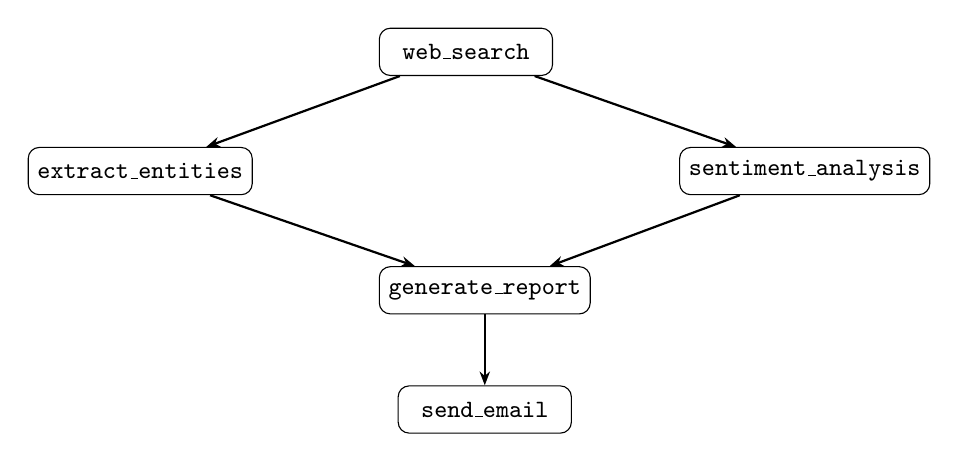
\begin{tikzpicture}[
    node distance=0.9cm and 1.6cm,
    every node/.style={draw, rounded corners, font=\small\ttfamily, minimum width=2.2cm, minimum height=0.6cm, fill=white},
    arr/.style={-{Stealth[length=5pt]}, thick}
]
\node (s1) {web\_search};
\node (s2) [below left=of s1] {extract\_entities};
\node (s3) [below right=of s1] {sentiment\_analysis};
\node (s4) [below right=of s2] {generate\_report};
\node (s5) [below=of s4] {send\_email};

\draw[arr] (s1) -- (s2);
\draw[arr] (s1) -- (s3);
\draw[arr] (s2) -- (s4);
\draw[arr] (s3) -- (s4);
\draw[arr] (s4) -- (s5);
\end{tikzpicture}
\end{center}

\noindent Step~1 (search) feeds into two parallel branches (steps 2--3), which merge at step~4 (report), followed by step~5 (email).
The model must plan the full 5-step pipeline, identify 5 tools from 8 candidates, correctly thread data between dependent steps, and recognize that entity extraction and sentiment analysis are independent given the search results.

\end{document}
